\chapter{Introduction}
\label{introduction}

\begin{abstract}
Sample Abstract.
\end{abstract}

\blfootnote{This chapter is partly based on \faFileTextO~\emph{M. Beller. Toward an
    Empirical Theory of Feedback-Driven Development, ICSE'18 (Student Research Competition)}~\cite{BellerSRC2018}.
}


\newpage

\dropcap{T}his is a introductory page.

\section{Background \& Context}
% In this thesis, you can reference pictures~\Cref{fig:devmodel} using Cleverref and circles \circled{5}.

% \begin{figure}[htb]
% 	\centering
% 	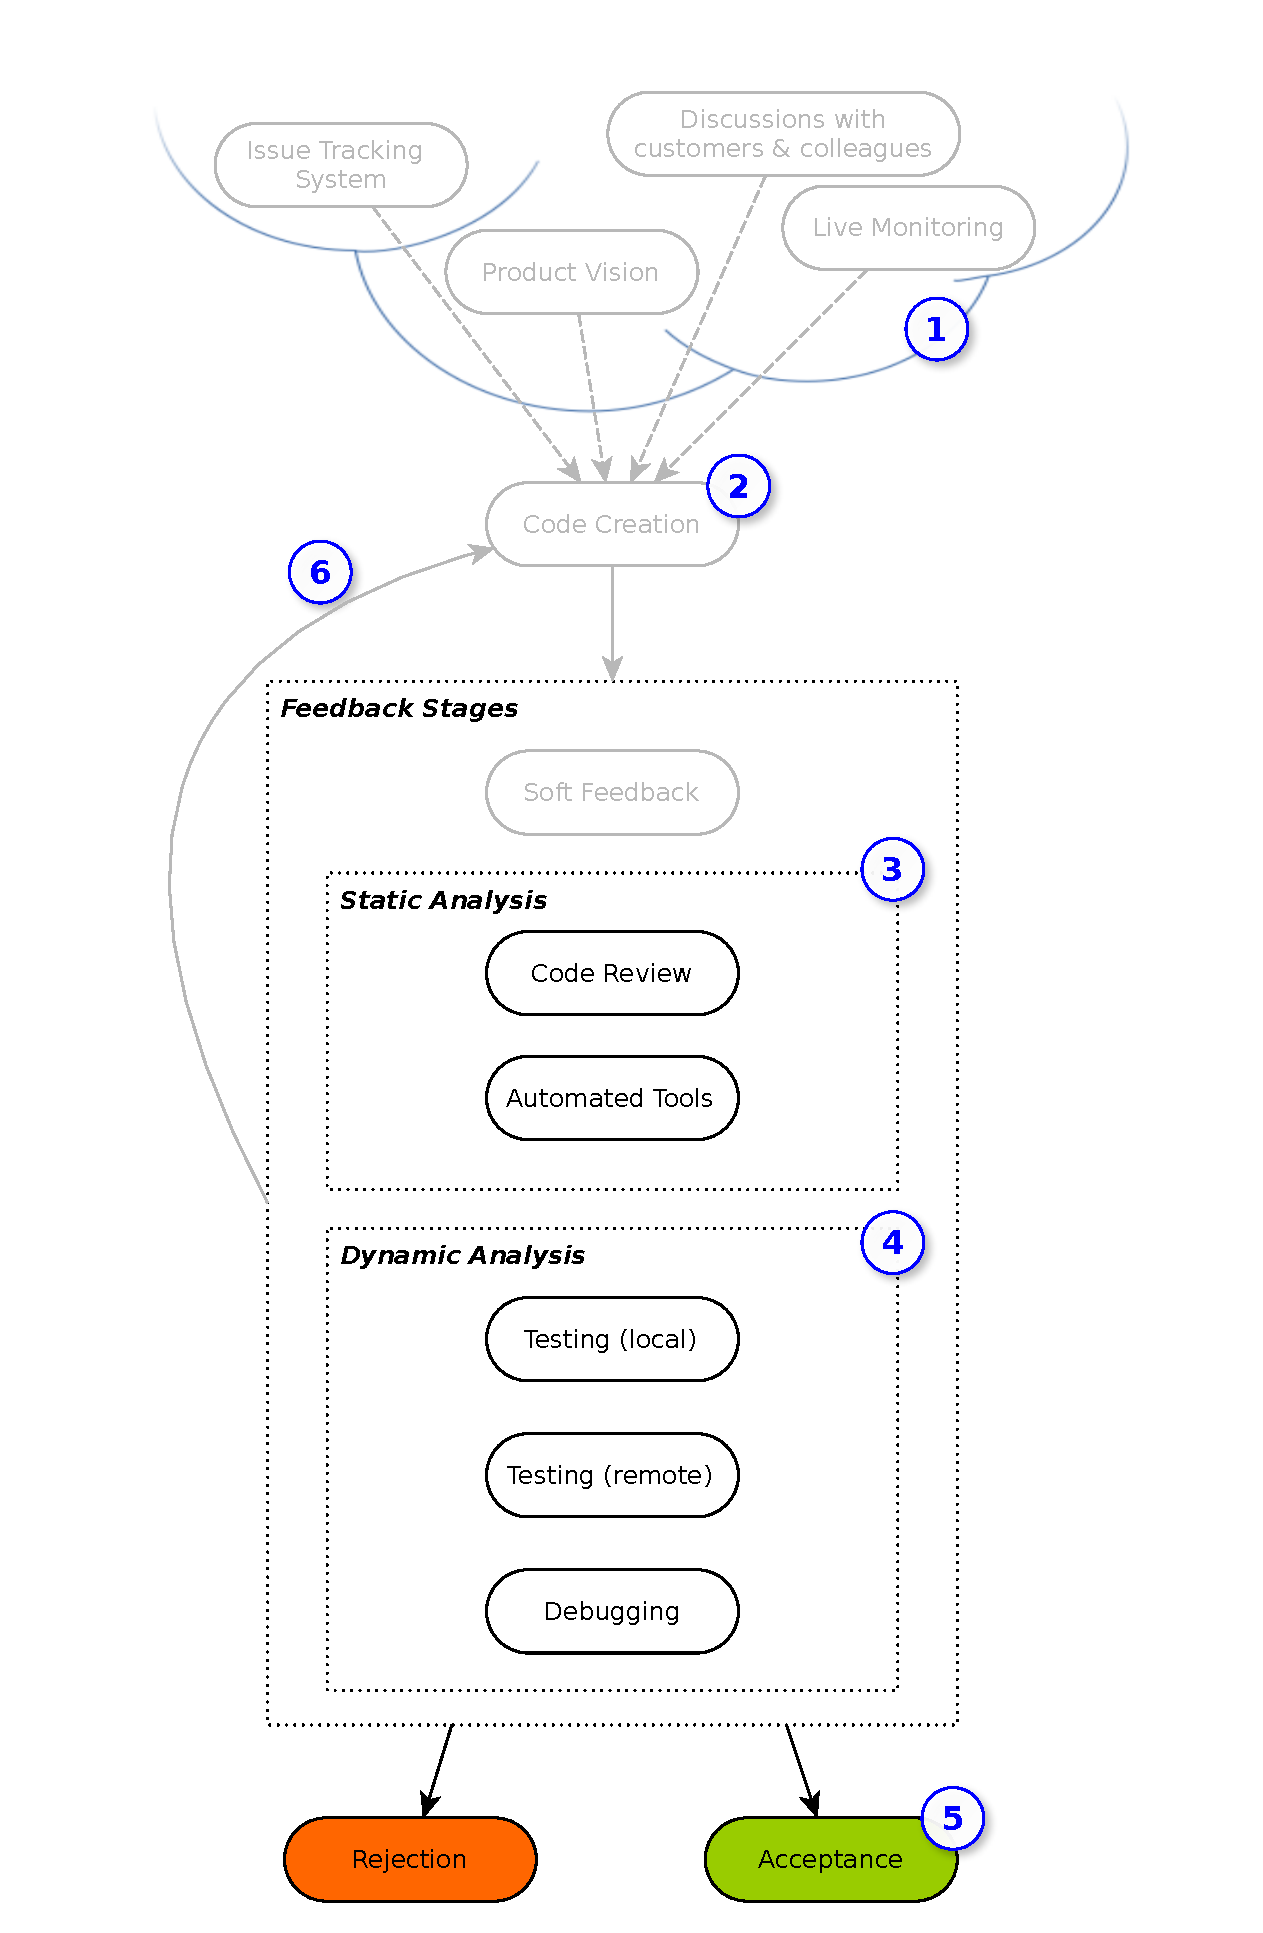
\includegraphics[width=0.65\columnwidth]{development_model_without_papers}
% 	\caption{The stages of the FDD model and their relationship to other
%           Software Engineering concepts.}
% 	\label{fig:devmodel}
% \end{figure}

We also have lists:

\begin{enumerate}
  \item Static Analysis~\circled{3} examines program artifacts or
    their source code without executing them~\cite{wichmann1995industrial}, while
 \item Dynamic Analysis~\circled{4} relies on information gathered from their
   execution~\cite{cornelissen2009systematic}.
\end{enumerate}

Or boxes:

\begin{framed}
This thesis is concerned with the empirical assessment of the state of the art of how developers
drive software development with the help of feedback loops. \cite{boyer2020dynamics}
\end{framed}

Or code:
\begin{lstlisting}[caption={\textsc{TrinityCore}},label={lst:e1}]
 x += other.x;
 y += other.y;
 z += other.y;
\end{lstlisting}


I hope this helps you get started!
Moritz

First time should be long: \gls{GCD}
Next time should be short: \gls{GCD}
